\documentclass[11pt,letterpaper]{article}
\usepackage[margin=1in]{geometry}
\usepackage{fontspec}
\usepackage{microtype,booktabs,graphicx,amsmath,longtable}
\usepackage[round,authoryear]{natbib}
\usepackage[font=small,labelfont=bf]{caption}
\usepackage[colorlinks=true,allcolors=blue]{hyperref}
\usepackage{xurl,setspace}
\setstretch{1.12}
\setlength{\emergencystretch}{2em}
\newcommand{\MTurkunemploymentestimate}{-9.5}
\newcommand{\MTurkunemploymentinparty}{79.3}
\newcommand{\MTurkunemploymentoutparty}{69.9}
\newcommand{\MTurkunemploymentCI}{[-12.5, -6.5]}
\newcommand{\MTurkinflationestimate}{-6.0}
\newcommand{\MTurkinflationinparty}{71.1}
\newcommand{\MTurkinflationoutparty}{65.2}
\newcommand{\MTurkinflationCI}{[-9.2, -2.8]}
\newcommand{\MTurkunemploymentbetterestimate}{-15.9}
\newcommand{\MTurkunemploymentbetterinparty}{61.9}
\newcommand{\MTurkunemploymentbetteroutparty}{46.0}
\newcommand{\MTurkunemploymentbetterCI}{[-21.1, -10.8]}
\newcommand{\MTurkinflationbetterestimate}{-9.2}
\newcommand{\MTurkinflationbetterinparty}{48.3}
\newcommand{\MTurkinflationbetteroutparty}{39.1}
\newcommand{\MTurkinflationbetterCI}{[-14.4, -4.1]}
\newcommand{\MTurkaverageestimate}{-7.7}
\newcommand{\MTurkaverageinparty}{75.2}
\newcommand{\MTurkaverageoutparty}{67.5}
\newcommand{\MTurkaverageCI}{[-10.3, -5.2]}
\newcommand{\MTurkN}{1,425}
\newcommand{\MTurkExport}{1,505}
\newcommand{\MTurkEligible}{1,503}
\newcommand{\MTurkNonpartisan}{78}
\newcommand{\MTurkScreen}{861}
\newcommand{\MTurkFlagged}{564}
\newcommand{\MTurkStrict}{1,258}
\newcommand{\Lucidunemploymentestimate}{-5.2}
\newcommand{\Lucidunemploymentinparty}{73.0}
\newcommand{\Lucidunemploymentoutparty}{67.9}
\newcommand{\LucidunemploymentCI}{[-10.6, 0.2]}
\newcommand{\Lucidinflationestimate}{-8.6}
\newcommand{\Lucidinflationinparty}{75.1}
\newcommand{\Lucidinflationoutparty}{66.5}
\newcommand{\LucidinflationCI}{[-14.2, -3.1]}
\newcommand{\Lucidunemploymentbetterestimate}{-6.0}
\newcommand{\Lucidunemploymentbetterinparty}{55.0}
\newcommand{\Lucidunemploymentbetteroutparty}{48.9}
\newcommand{\LucidunemploymentbetterCI}{[-13.9, 1.9]}
\newcommand{\Lucidinflationbetterestimate}{-10.4}
\newcommand{\Lucidinflationbetterinparty}{59.4}
\newcommand{\Lucidinflationbetteroutparty}{49.0}
\newcommand{\LucidinflationbetterCI}{[-18.3, -2.6]}
\newcommand{\Lucidaverageestimate}{-6.9}
\newcommand{\Lucidaverageinparty}{74.1}
\newcommand{\Lucidaverageoutparty}{67.2}
\newcommand{\LucidaverageCI}{[-11.8, -2.1]}
\newcommand{\LucidN}{624}
\newcommand{\LucidExport}{821}
\newcommand{\LucidEligible}{794}
\newcommand{\LucidNonpartisan}{170}
\newcommand{\LucidScreen}{529}
\newcommand{\LucidFlagged}{95}
\newcommand{\LucidStrict}{467}

\makeatletter\let\inputtable\@@input\makeatother
\title{An Unclear Gap:\\Partisan Cues and Evaluations of\\the Same Economic Information}
\author{Carolyn E. Roush \and Gaurav Sood}
\date{October 2026}
\hypersetup{pdfauthor={Carolyn E. Roush and Gaurav Sood},pdftitle={An Unclear Gap: Partisan Cues and Evaluations of the Same Economic Information}}
\begin{document}
\maketitle
\begin{abstract}
\noindent Does giving people the same economic figures lead them to the same assessment? Two survey experiments present small declines in unemployment and inflation under either a Democratic President Obama cue or a Republican Congress cue. Respondents classify the changes as ``got better,'' ``stayed about the same,'' or ``got worse.'' People rated the same numerical changes less favorably when the question mentioned the opposing party. On a scale assigning these responses 100, 50, and 0, respectively, the unemployment and inflation effects are \MTurkunemploymentestimate{} and \MTurkinflationestimate{} points on MTurk and \Lucidunemploymentestimate{} and \Lucidinflationestimate{} points on Lucid. This shows that partisan context affects how people describe economic performance, but leaves open whether they see the changes differently or simply answer in ways that favor their party.
\end{abstract}
\vspace{1em}
\noindent\small Replication materials: \url{https://github.com/soodoku/unclear_gap}. All estimates, tables, and figures are generated from the accompanying public extracts.\normalsize
\newpage
\section{What a partisan gap can mean}
When Democrats and Republicans give different answers to a question about the economy, the difference need not arise entirely from different factual beliefs. Respondents may disagree about what happened, how much the change matters, or which response best describes it. A question asking whether conditions ``got better'' leaves room for evaluation even when it supplies numerical information.

This distinction matters for interpreting partisan gaps on surveys. Work on partisan survey response separates factual beliefs from the incentives and judgments involved in reporting them \citep{bullock2019}. Research on Iraq likewise distinguishes beliefs about events from interpretations of those events \citep{gaines2007}. Our companion study examines the prevalence and measurement of partisan knowledge gaps across survey items \citep{roush2023}. Here we examine a narrower question: does the partisan context of an economic question change how respondents evaluate the same supplied numerical changes?

We use two experiments that hold the numerical changes and response categories fixed while varying whether the question invokes President Obama or a Republican-controlled Congress. We compare the cue associated with a respondent's opposing party with the cue associated with their own party. If evaluations depend only on the supplied numbers, this comparison should produce no difference. A difference demonstrates sensitivity to the cue package. It does not, by itself, reveal whether respondents understood or believed the numbers, changed their standards for a meaningful improvement, or used the answer to express support for a party.

The design also leaves response-option vagueness unmanipulated. ``Stayed about the same'' plausibly permits different thresholds for a meaningful change, but these experiments cannot tell us whether more precise options would reduce the cue effect. We therefore treat vagueness as a possible explanation and a question for further experimentation, rather than the treatment whose effect we estimate.

\section{Design and data}
\subsection{Two cue packages, the same numerical changes}
The MTurk survey was fielded on June 29, 2020, and the Lucid survey on January 27, 2023. The MTurk instrument recruited US adults and offered a payment of \$0.75. Both are nonprobability online samples. The available data include no survey weights, and the estimates describe the participating analytic samples rather than the US electorate.

The study documentation describes random assignment to an Obama condition or a Republican Congress condition. The recorded assignment and arm-specific answers are mutually consistent. The release includes the fielded questionnaire text, but the available materials do not contain the randomizer settings or assignment logs. Causal interpretation relies on assignment having been implemented as described.

The experiments appeared after other partisan questions. On MTurk, respondents first assessed the prior year's economy and predicted how Democrats and Republicans would assess the economy, unemployment, and inflation; the introduction explicitly asked how the parties would interpret ``the same information.'' Lucid included earlier questions linking party affiliation with racial or religious groups. These preceding questions may make partisan interpretation salient or suggest how respondents are expected to answer. The randomized comparisons remain comparisons within the administered surveys, but the design does not identify how the cue effects would differ without that preceding context.

The unemployment prompt stated a decline from 5.0\% to 4.8\%. The Obama version referred to President Obama's last year in office, 2016; the Republican version referred to 2016, when Republicans controlled both houses of Congress. The inflation prompt stated a decline from 2.1\% to 1.9\%. In the MTurk instrument, the inflation question followed the partisan context established earlier without repeating the actor; the Lucid inflation prompt repeated the Obama or Congress cue. Thus, the second study repeats the central contrast, with a difference in how explicitly the cue is carried into the inflation item. Full wording appears in the replication materials.

These are the \emph{supplied survey figures}, not verified year-end descriptions of the 2016 economy. The cited official series report December 2016 unemployment of 4.7\%, and twelve-month CPI inflation rising from 0.7\% in December 2015 to 2.1\% in December 2016 \citep{blsjobs,blscpi}. This discrepancy limits a factual-knowledge interpretation. It does not change the fact that the two randomized arms within each study supplied the same numerical changes.

Both items offered ``got better,'' ``stayed about the same,'' and ``got worse.'' Neither instrument tested comprehension or recall of these economic figures after presenting them. Moreover, a small decline in inflation need not be judged desirable by every informed respondent. We therefore analyze evaluations without designating any response objectively correct.

The contrast changes more than a party label. It changes a named president into a legislature, along with the emphasis of the wording. For Democrats, Obama is the own-party cue and Congress the opposing-party cue; for Republicans, the mapping is reversed. The pooled estimate averages those two comparisons. It cannot isolate a pure party-label effect from actor, institutional, or wording effects.

\subsection{Analytic samples and screening}
The MTurk export contains \MTurkExport{} records, of which \MTurkEligible{} consented and have an assignment and both outcomes. Excluding respondents without a Democratic or Republican identification, including a lean toward either party, leaves \MTurkN{} partisans. The Lucid export contains \LucidExport{} records after removing the export's metadata rows. Excluding previews and nonconsenting records leaves \LucidEligible{} assigned respondents with outcomes; \LucidN{} are partisans under the provider's party coding. Neither main partisan sample has missing outcomes.

We use all eligible partisans for the main estimates. We also report the previously used screening rules as sensitivity analyses. On MTurk, a record is flagged if an existing IP review flagged its address or if at least two of six low-incidence or unusual responses were present: very short or long sleep, a prosthetic limb, a vision impairment, a hearing impairment, gang membership, or a family member's gang membership. These questions followed the experiment. The screen is a heuristic and does not establish that a respondent is fraudulent or inattentive. In particular, the vision and hearing items asked about impairments broadly. The screen retains \MTurkScreen{} partisans and flags \MTurkFlagged{}.

Lucid included an instructed-response check before the economic experiment. Passing required selecting exactly the two requested response options. It retains \LucidScreen{} partisans and flags \LucidFlagged{}. The timing is more favorable for a subgroup analysis than the MTurk screen, but passing still defines a different target population. We also report strict party identifiers, excluding leaners, and estimates clustered by the original IP address using anonymous group identifiers. Sharing an address does not establish that two records belong to the same person; we do not delete records solely on that basis.

\section{Estimands and inference}
We score ``got worse'' as 0, ``stayed about the same'' as 50, and ``got better'' as 100. The mean score is a compact summary of the ordered responses that assumes equal spacing. To show results without that assumption, we separately analyze the probability of choosing ``got better'' and release the complete response distributions.

For each study and outcome, let $\bar Y_{p,o}$ and $\bar Y_{p,i}$ be the mean outcome among respondents identifying with party $p$ who received the opposing-party and own-party cues. Let $w_p$ be party $p$'s share of the relevant analytic sample. Our estimand is
\[
\widehat\tau = \sum_{p\in\{D,R\}} w_p\left(\bar Y_{p,o}-\bar Y_{p,i}\right).
\]
A negative value indicates less favorable evaluations under the opposing-party cue. Standardizing to the same party shares in both arms prevents chance differences in party composition from contributing to the pooled comparison. Each sensitivity sample uses its own party shares. The weights are sample composition weights, not population survey weights.

We compute variances from the four independent party-by-cue cell means, treating party shares as fixed, and use a Welch--Satterthwaite approximation for two-sided 95\% confidence intervals. This variance agrees with a saturated cell-means regression using HC2 standard errors. The four primary score comparisons---two outcomes in each study---also receive Holm-adjusted $p$-values. Binary outcomes, party-specific estimates, and screening checks are secondary analyses; their intervals are unadjusted.

The two outcomes come from the same respondents and are analyzed separately. A supplementary respondent-level average preserves their covariance. Additional checks permute the cue assignment within party, conditional on the observed arm counts, and cluster uncertainty by anonymous IP group. Permutation inference assumes exchangeability within party under the documented randomization. The analysis was reconstructed from the available data and instruments; no preregistration or prespecified analysis plan was available.

\section{Results}
\subsection{Evaluations shift with the cue}
Table~\ref{tab:main} reports the main comparisons. On MTurk, the unemployment evaluation falls from \MTurkunemploymentinparty{} under the own-party cue to \MTurkunemploymentoutparty{} under the opposing-party cue: a difference of \MTurkunemploymentestimate{} points (95\% CI \MTurkunemploymentCI{}). The inflation difference is \MTurkinflationestimate{} points (\MTurkinflationCI{}). These are differences on the evaluation scale, not percentage-point changes in the probability of giving any particular answer.

\begin{table}[htbp]
\centering\small
\caption{Evaluations under own-party and opposing-party cues}\label{tab:main}
\begin{tabular}{llrrrrl}\toprule
Study & Outcome & $N$ & Own & Opposing & Difference & 95\% CI\\\midrule
\inputtable{../tabs/main.tex}
\bottomrule\end{tabular}
\par\smallskip\raggedright\footnotesize All eligible partisans, including leaners. Means are standardized to each study's observed party shares. Scores: worse = 0, same = 50, better = 100. Difference is opposing minus own. Intervals use independent cell variances and Welch--Satterthwaite degrees of freedom.
\end{table}

The Lucid inflation difference is also negative: \Lucidinflationestimate{} points (\LucidinflationCI{}). Its unemployment estimate is \Lucidunemploymentestimate{} points (\LucidunemploymentCI{}). That interval includes zero and also permits a substantively noticeable negative effect. It is neither decisive evidence of a cue effect on this item nor strong evidence that the cue does not matter. Holm adjustment across the four primary comparisons leaves the other three distinguishable from zero at the conventional level; the Lucid unemployment comparison remains uncertain.

\subsection{How often respondents say ``got better''}
The binary comparison makes the behavioral meaning of these differences easier to see (Table~\ref{tab:binary}). On MTurk, the unemployment ``got better'' share is \MTurkunemploymentbetterinparty{}\% under the own-party cue and \MTurkunemploymentbetteroutparty{}\% under the opposing-party cue. The difference is \MTurkunemploymentbetterestimate{} percentage points (\MTurkunemploymentbetterCI{}). For inflation, the difference is \MTurkinflationbetterestimate{} percentage points (\MTurkinflationbetterCI{}).

On Lucid, the corresponding differences are \Lucidunemploymentbetterestimate{} percentage points for unemployment (\LucidunemploymentbetterCI{}) and \Lucidinflationbetterestimate{} for inflation (\LucidinflationbetterCI{}). The uncertainty pattern resembles that for the score: the unemployment contrast on Lucid is less conclusive. The binary results show that the score differences are not merely an artifact of assigning equal distances to the three categories.

\begin{table}[htbp]\centering\small
\caption{Probability of selecting ``got better''}\label{tab:binary}
\begin{tabular}{llrrl}\toprule
Study & Outcome & Own (\%) & Opposing (\%) & Difference in pp [95\% CI]\\\midrule
\inputtable{../tabs/binary.tex}
\bottomrule\end{tabular}
\par\smallskip\raggedright\footnotesize Same sample and party standardization as Table~\ref{tab:main}. Secondary comparisons; intervals are unadjusted for multiplicity.
\end{table}

\subsection{Screening and other sensitivity checks}
The screen-passed samples yield larger negative point estimates for both items in both studies (Figure~\ref{fig:effects}; Appendix Table~\ref{tab:sensitivity}). This pattern is consistent with screening removing responses that dilute the contrast, but it does not establish that interpretation. Respondents who pass differ from those who fail, and the MTurk screen is measured after treatment. Conditioning on it can select respondents differently across arms. We therefore retain the full-sample comparisons as primary and show the screening results without equating passing with truthfulness.

\begin{figure}[htbp]\centering
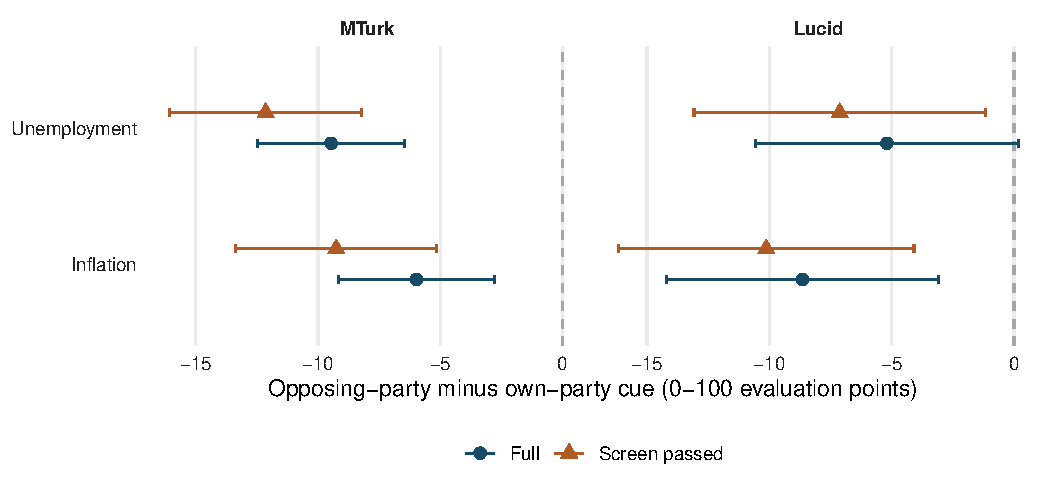
\includegraphics[width=\linewidth]{../figs/effects.pdf}
\caption{Cue effects in full and screen-passed samples. Points show opposing-party minus own-party differences on the 0--100 evaluation scale; bars show unadjusted 95\% confidence intervals. The MTurk screen uses post-experiment responses. Each sample is standardized to its own party composition.}\label{fig:effects}
\end{figure}

Party-specific estimates are reported in Appendix Table~\ref{tab:party}. They describe separate randomized cue contrasts within each respondent-party group; a comparison of Democrats with Republicans is not itself randomized. Clustering by IP group leaves the main interval pattern unchanged. No single observation reverses any main point estimate. The replication files report these checks, within-party permutation results, and strict-identifier estimates so that the findings can be assessed without relying on a particular screen.

\section{What we learn}
Supplying the same numerical changes does not eliminate partisan context from economic evaluations. In these samples, respondents generally give less favorable assessments when the question foregrounds an actor from the opposing party. The strongest evidence concerns both MTurk items and the Lucid inflation item; the Lucid unemployment contrast remains imprecise. The findings make it difficult to interpret every partisan difference on a broad evaluative question as a difference in stored factual knowledge.

The experiment does not show that knowledge is identical across respondents. People may ignore or disbelieve the supplied numbers, bring different background information to the task, apply different standards, or express political loyalties through their answers. Neither comprehension nor incentives for accurate reporting were manipulated here. Similarly, the design does not establish that respondents blame or credit the named actor: it establishes a response to the cue package, which also changes institution and wording.

Vague categories remain a plausible contributor. A decline can be numerically real yet small enough for someone to call it ``about the same,'' and ``better'' additionally asks for a judgment about desirability. To test whether this latitude produces the cue effect, a subsequent experiment would need to randomize precise versus evaluative response formats while holding the cue and information fixed. Direct recall or comprehension measures would help distinguish common exposure from common knowledge; incentives could help distinguish sincere assessments from expressive responding. Those are identifiable next questions, rather than conclusions supplied by the present data.

\bibliographystyle{apalike}
\bibliography{references}
\clearpage
\appendix
\section{Sample and party sensitivity}
\begin{table}[htbp]\centering\small
\caption{Cue effects across analytic samples}\label{tab:sensitivity}
\begin{tabular}{lllrl}\toprule
Study & Sample & Outcome & $N$ & Difference [95\% CI]\\\midrule
\inputtable{../tabs/sensitivity.tex}
\bottomrule\end{tabular}
\par\smallskip\raggedright\footnotesize Evaluation-score points, opposing minus own. Full includes leaners; strict identifiers excludes them. The MTurk screen combines the supplied IP flag with post-experiment responses; the Lucid screen is an earlier instructed-response check. Each row uses that sample's party shares. These are overlapping samples, not independent replications.
\end{table}
\begin{table}[htbp]\centering\small
\caption{Cue effects by respondent party}\label{tab:party}
\begin{tabular}{lllrl}\toprule
Study & Party & Outcome & $N$ & Difference [95\% CI]\\\midrule
\inputtable{../tabs/party.tex}
\bottomrule\end{tabular}
\par\smallskip\raggedright\footnotesize Full eligible samples, including leaners. Differences are in score points. Party identification is not randomized. For Democrats the contrast is Congress minus Obama; for Republicans it is Obama minus Congress. Intervals are unadjusted secondary comparisons.
\end{table}
\end{document}
